%
% The first command in your LaTeX source must be the \documentclass command.
\documentclass[sigplan,screen]{acmart}

%
% defining the \BibTeX command - from Oren Patashnik's original BibTeX documentation.
\def\BibTeX{{\rm B\kern-.05em{\sc i\kern-.025em b}\kern-.08emT\kern-.1667em\lower.7ex\hbox{E}\kern-.125emX}}
    
% Rights management information. 
% This information is sent to you when you complete the rights form.
% These commands have SAMPLE values in them; it is your responsibility as an author to replace
% the commands and values with those provided to you when you complete the rights form.
%
% These commands are for a PROCEEDINGS abstract or paper.
\copyrightyear{2018}
\acmYear{2018}
\setcopyright{acmlicensed}
\acmConference[Woodstock '18]{Woodstock '18: ACM Symposium on Neural Gaze Detection}{June 03--05, 2018}{Woodstock, NY}
\acmBooktitle{Woodstock '18: ACM Symposium on Neural Gaze Detection, June 03--05, 2018, Woodstock, NY}
\acmPrice{15.00}
\acmDOI{10.1145/1122445.1122456}
\acmISBN{978-1-4503-9999-9/18/06}

%
% These commands are for a JOURNAL article.
%\setcopyright{acmcopyright}
%\acmJournal{TOG}
%\acmYear{2018}\acmVolume{37}\acmNumber{4}\acmArticle{111}\acmMonth{8}
%\acmDOI{10.1145/1122445.1122456}

%
% Submission ID. 
% Use this when submitting an article to a sponsored event. You'll receive a unique submission ID from the organizers
% of the event, and this ID should be used as the parameter to this command.
%\acmSubmissionID{123-A56-BU3}

%
% The majority of ACM publications use numbered citations and references. If you are preparing content for an event
% sponsored by ACM SIGGRAPH, you must use the "author year" style of citations and references. Uncommenting
% the next command will enable that style.
%\citestyle{acmauthoryear}

%
% end of the preamble, start of the body of the document source.
\begin{document}

%
% The "title" command has an optional parameter, allowing the author to define a "short title" to be used in page headers.
\title{Agile Inter-team Software Development}

%
% The "author" command and its associated commands are used to define the authors and their affiliations.
% Of note is the shared affiliation of the first two authors, and the "authornote" and "authornotemark" commands
% used to denote shared contribution to the research.


\author{Sarthak Tiwari}
\affiliation{%
  \department{School of Computing, Informatics, and Decision Systems Engineering}
  \institution{Arizona State University}
  \city{Tempe}
  \state{Arizona}
  \country{USA}}
\email{sarthak.tiwari@asu.edu}

\author{Ruben Acu{\~n}a}
\affiliation{%
  \department{School of Computing, Informatics, and Decision Systems Engineering}
  \institution{Arizona State University}
  \city{Tempe}
  \state{Arizona}
  \country{USA}}
\email{ruben.acuna@asu.edu}



%
% By default, the full list of authors will be used in the page headers. Often, this list is too long, and will overlap
% other information printed in the page headers. This command allows the author to define a more concise list
% of authors' names for this purpose.
\renewcommand{\shortauthors}{Tiwari and Acu{\~n}a}


\settopmatter{printacmref=false}						%RA: get rid of dumb ACM reference format BLAH BLAH

%
% The abstract is a short summary of the work to be presented in the article.
\begin{abstract}

With the boom in the use of agile process model, imperfect implementations of agile are frequently being seen, out of which the problem of inter-team communication in agile teams is one of the most common issue.
An agile team by its definition is a group of people who are self-sufficient to bring their responsibilities to closure, the interaction between different teams is thus considered minimal in most projects implementing agile.
This causes problems when the integration of end-products of different teams is carried out.
In this paper we have taken a detailed look at this problem and how we can mitigate this.

\end{abstract}

%
% The code below is generated by the tool at http://dl.acm.org/ccs.cfm.
% Please copy and paste the code instead of the example below.
%
\begin{CCSXML}
<ccs2012>
 <concept>
  <concept_id>10010520.10010553.10010562</concept_id>
  <concept_desc>Computer systems organization~Embedded systems</concept_desc>
  <concept_significance>500</concept_significance>
 </concept>
 <concept>
  <concept_id>10010520.10010575.10010755</concept_id>
  <concept_desc>Computer systems organization~Redundancy</concept_desc>
  <concept_significance>300</concept_significance>
 </concept>
 <concept>
  <concept_id>10010520.10010553.10010554</concept_id>
  <concept_desc>Computer systems organization~Robotics</concept_desc>
  <concept_significance>100</concept_significance>
 </concept>
 <concept>
  <concept_id>10003033.10003083.10003095</concept_id>
  <concept_desc>Networks~Network reliability</concept_desc>
  <concept_significance>100</concept_significance>
 </concept>
</ccs2012>
\end{CCSXML}

\ccsdesc[500]{Computer systems organization~Embedded systems}
\ccsdesc[300]{Computer systems organization~Redundancy}
\ccsdesc{Computer systems organization~Robotics}
\ccsdesc[100]{Networks~Network reliability}

%
% Keywords. The author(s) should pick words that accurately describe the work being
% presented. Separate the keywords with commas.
\keywords{Agile, Software Engineering, Software Development, Process Models, Inter-team, Management}

%
% This command processes the author and affiliation and title information and builds
% the first part of the formatted document.
\maketitle

\section{Introduction}
%Introduction (Introducing the topic)

%AM: What is the problem?
%introduce the need to scale to multiple agile teams
Agile approaches are popular in software development for numerous reasons.
However, the structure of the agile process does not lend itself to large teams and is not suitable for large projects.
With the growth in complex software, situations arise where multiple agile teams need to work together to achieve a common goal.
%thesis statement
When scaling to parallel agile teams, the most important consideration is quality communication, both personal and architectural.
%
For an example of a company developing a complex piece of software, consider Spotify AB who has over 30 teams \cite{kniberg12}.
Spotify is a streaming music client which supports media, commercial, and social features.
The basic element of development organization at Spotify is the Squad, analogous to a Scrum team.
%Each Squad is the autonomous developer, with a localized working area, of a particular sub-system in the product.
Squads in related areas are grouped together into Tribes. 
The overall structure is illustrated in Figure~\ref{fig:spotify_structure}.
\begin{figure}[h]
  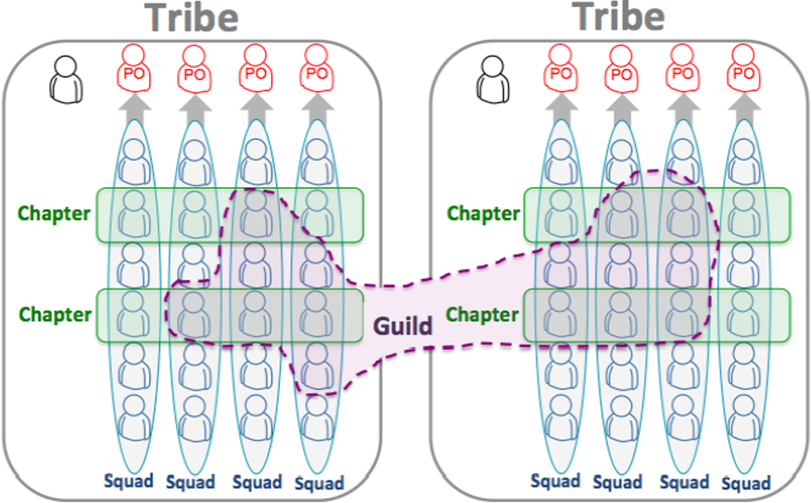
\includegraphics[width=\linewidth]{images/kniberg12_structure.png}
  \caption{Agile team organization at Spotify \cite{kniberg12}.}
  \label{fig:spotify_structure}
\end{figure}


%AM: Why is it interesting/important?
%introduce agile
As outlined in the Agile Manifesto \cite{beck2001agile}, an agile process gives individuals and interactions value over processes and tools.
An agile team should contain all that is required for them to do their work, thus interactions are intensely intra-team.
However, diverse feature sets such as required in the Spotify application necessitate many skillsets and substantial manpower.
By moving to a multi-team model, complex projects can benefit from agility, provided that the process is adapted.
%personal communication
Multiple teams increases the importance of communication, from simple interpersonal communication to system specification. 
The agile approach of interacting in-person can fail due to reasons such as the vertical structure of the company organization and layers of middle managers \cite{dzone_article}.
The large number of intermediaries can cause an agile process to breakdown as it takes longer than usual time for messages to reach their destination than can afforded.
%arch communication
In an agile process, where Big Design Up-front may typically be avoided, the move to multiple teams motivates a need to communicate design decisions.
%todo: component boundaries?
For successful integration of technological components, system elements must have well defined functional specifications, and interfaces.

%RA: feel like we can skip AM suggest section on Why is it hard.
%AM: What are the key components of [the] proposed approach? Also include assumptions/limitations
%We discuss approaches, which if implemented correctly, provide a more robust and functional process for inter-team agile development. 

%outline of rest of paper
This document is organized as follows: Introduction, Communication Concerns, Supporting Communication in Inter-team Development, and Conclusion. 
In Section ~\ref{sec:spt_ex}, we discuss example communication concerns in an agile project.
In Section ~\ref{sec:prop_appro}, we present some process adaptations that can help to resolve issues.
Lastly, Section ~\ref{sec:conclusion} concludes with an overview of important aspects of inter-team agile development.


%This problem is difficult to fix as this is so embedded in the working agile culture of the current organizations that changing them will take a long time, thus an immediate patch that works is required. %RA: this is an important observation, just too detailed for intro. 

\section{Spotify: A Canonical Example} 
\label{sec:spt_ex} 
For an example of a company using many agile teams, consider Spotify who has over 30 teams \cite{kniberg12}.
The basic element of development organization at Spotify is the Squad, analogous to a Scrum team.
Each Squad is the autonomous developer, with a localized working area, of a particular sub-system in the product.
Squads in related areas are grouped together into Tribes. 
The overall structure is illustrated in Figure~\ref{fig:spotify_structure}.
Although larger than Squads (7-10 members), Tribes are limited in size (< 100) to ensure smooth communication.

\begin{figure}[h]
  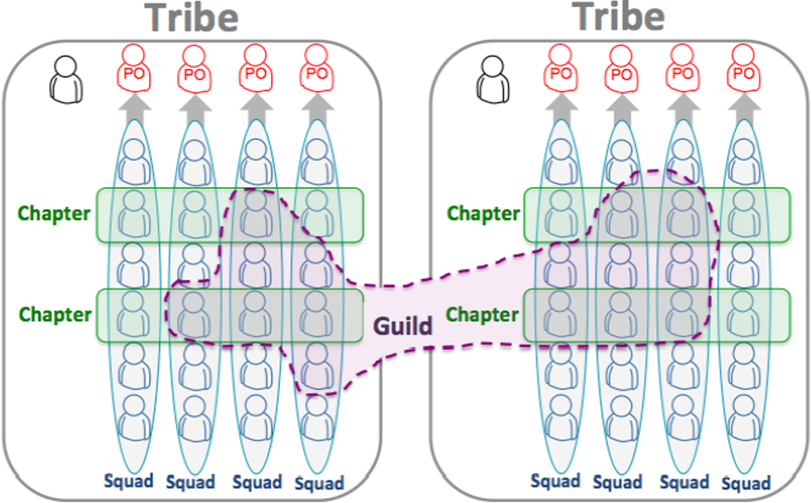
\includegraphics[width=\linewidth]{images/kniberg12_structure.png}
  \caption{Agile team organization at Spotify \cite{kniberg12}.}
  \label{fig:spotify_structure}
\end{figure}


\subsection{Communication at Spotify}
%social fixes
A fundamental issue with tasking teams with different goals is that teams can become isolated with respect to the context of their work.
At Spotify \cite{kniberg12}, offices are laid out so that the Squads making up a Tribe are spatially close. This leads to an environment where an informal exchange of information on the Tribes work will occur.
%second problem
Consider another scenario: a tester on a particular agile team invests time to solve a particular problem, which is also faced by another tester on a different team. Without communication, these team members would perform redundant work.
To address this problem Spotify defines Chapters \cite{kniberg12}, which are crosscutting divisions which gathers individuals with similar roles across different Squads. 


\section{Communication in Inter-team Development}
\label{sec:prop_appro} 
The general problem of communication can be tackled from two perspectives.
First, stakeholders at different levels need to have ways to pass information.
This can be addressed by adaptions in development process and leveraging technology.
Second, the quality of communication needs to be accurate.
This can be addressed by sound system specification through architecture and design.
%In Section ~\ref{sec:proc_impv}, we discuss the adaptations to an agile process, and team structure, to support better collaboration between teams.
%In Section ~\ref{sec:tech_impv}, we discuss the ways in which technology improve inter-team communication
%In Section ~\ref{sec:imp_of_dsgn}, we discuss the role of architecture and design in mitigating communication issues.

\subsection{Process Improvements} 
\label{sec:proc_impv}
	There are many small changes \cite{collabAcrossAgile_article} that we can incorporate in our process model to make sure that parallel developing agile teams do not run into problems when they reach the integration phase.
	These changes are to be made part of the entire process and are not to be implemented only in the end.

%Changes in standups
	One of the most critical aspect of agile process model is to have daily standups which are the platform serving the purpose of letting each team member know the work being done in the other parts of the team and correlate it with the work being done by them.
	This results in escalation of differences between the development early in the process and prevents end moment discovery of mismatches in interfaces and such.
	In the case of multiple agile teams this problem is compounded as usually a daily stand up is a closed activity of the team itself, thus preventing other teams from knowing the results or discussions of each other.
	This can be resolved by having a representative of each concerned team being present in the daily standup thus letting each team know the status of other teams.

%Changes to Product Owner
Though in usual implementations the product owner is responsible for agile teams under his supervision, in large projects with multiple agile teams where a number of product owners are present sometimes over time the vision of the owners may get too distinct from each other thus pushing the development track in different directions.
This can be limited by having regular meetings of product owners where the scope and vision of the project could be synced again. This can be a bi-weekly or monthly meeting depending on the size of the project.

%Changes in Planning Sessions
All the initial, intermediate and final planning sessions should be made such that all the teams which are or could be impacted by that part of the project are part of the meeting.
This can assist in early agreement on high-level requirements and standardization of inter-team interfaces.

\subsection{Technology Approaches} \label{sec:tech_impv}
Selecting an appropriate technology stack plays an important role maintaining a widely distributed team.
Technology can help teams in keeping track of things that they need to do so that other teams can work efficiently.
The following are some of the areas where the technology can enable a more efficient agile process environment.

%Communication Tools
Since agile focuses on personal interaction, particularly face-to-face conversation, video conferencing tools can help the team interactions become more fluid and clearer.
They also make the communication real-time thus removing the delay in process due to time spent in communicating ideas across teams.
%Integration Tools
Continuous integration tools can go a long way in finding out inter-team problems early in the process as every time any team makes a change, its impact on the entire project can be seen.

\subsection{Importance of Architecture/Design}\label{sec:imp_of_dsgn}
%Why is Design/Architecture so important when doing this?

As we know that the product owner in an agile process model is the person with the vision of what the project will look like and if it is a small team the product owner can clearly pass this to each and every member of the team and even each member can query the product owner directly when in doubt.
But in large scale projects where multiple agile teams are working together in supervision of a few product owners it is practically impossible for the owner to keep doing what they did in a small team, that’s where a formal definition of their vision comes in handy as it enables the teams to look up to something when encountering a design decision.
The design or architecture in this case acts as a common vision for not only the teams but also for the communication between all the product owners.
The design acts as a “deadlock breaker in decisions” \cite{architecureRole_article} as when the teams can’t come to a common consensus the design shows the path to take.
%non specification fix
Spotify addresses this issue with a more organizational approach by defining a "system owner" role \cite{kniberg12}.
This role is more casual than an architect role, and focuses on defining a "go-to" person who can maintain long term stewardship over a sub-system. 

In addition to specification of system elements, architecture can also be used to empower teams.
As discussed by Parnas \cite{Parnas72}, there are two general approaches to decomposing systems: 1) compartmentalizing a computational process and, 2) focusing on information hiding.
The latter approach ideal for agile development since this approaches defines system components in terms of design decisions, which empowers individual teams.

\section{Conclusion}\label{sec:conclusion}
As we have seen, inter-team communication can be an obstacle in agile teams working on the same thing as intermediaries in communication and lack of common personal causes things to go haywire if left unchecked.
To reduce this problem a number of small additions can be done to the process as specified but the most important part of the change is a good architecture and design which is available to all the teams and thus provides a common framework to all the teams involved.

\section{CCS Concepts and User-Defined Keywords}

Two elements of the ``acmart'' document class provide powerful taxonomic tools for you to help readers find your work in an online search. 

The ACM Computing Classification System --- \url{https://www.acm.org/publications/class-2012} --- is a set of classifiers and concepts that describe the computing discipline. Authors can select entries from this classification system, via \url{https://dl.acm.org/ccs/ccs.cfm}, and generate the commands to be included in the \LaTeX\ source. 

User-defined keywords are a comma-separated list of words and phrases of the authors' choosing, providing a more flexible way of describing the research being presented.

CCS concepts and user-defined keywords are required for all short- and full-length articles, and optional for two-page abstracts. 

%
% The next two lines define the bibliography style to be used, and the bibliography file.
\bibliographystyle{ACM-Reference-Format}
\bibliography{sample-base}

\end{document}
